\chapter{操作方法}

\section{\tacsim の画面}

図\ref{fig:ch3-tacsim}に\tacsim の画面を示す. ①には\tac のコンソールが描画されており, 実機と同じようにスイッチとボタンを使用することができる(実機の操作方法は\url{https://github.com/tctsigemura/TeC7/blob/master/Doc/Manual/manual.pdf}を参考のこと). ②にはマイクロSDの代わりに使用するディスクイメージの読み込みボタンやレジスタの内容出力, ブレークポイントの設定といったデバッグ用の機能が表示されている. ③は\tacsim のターミナルである.

\begin{figure}[H]
    \centering
    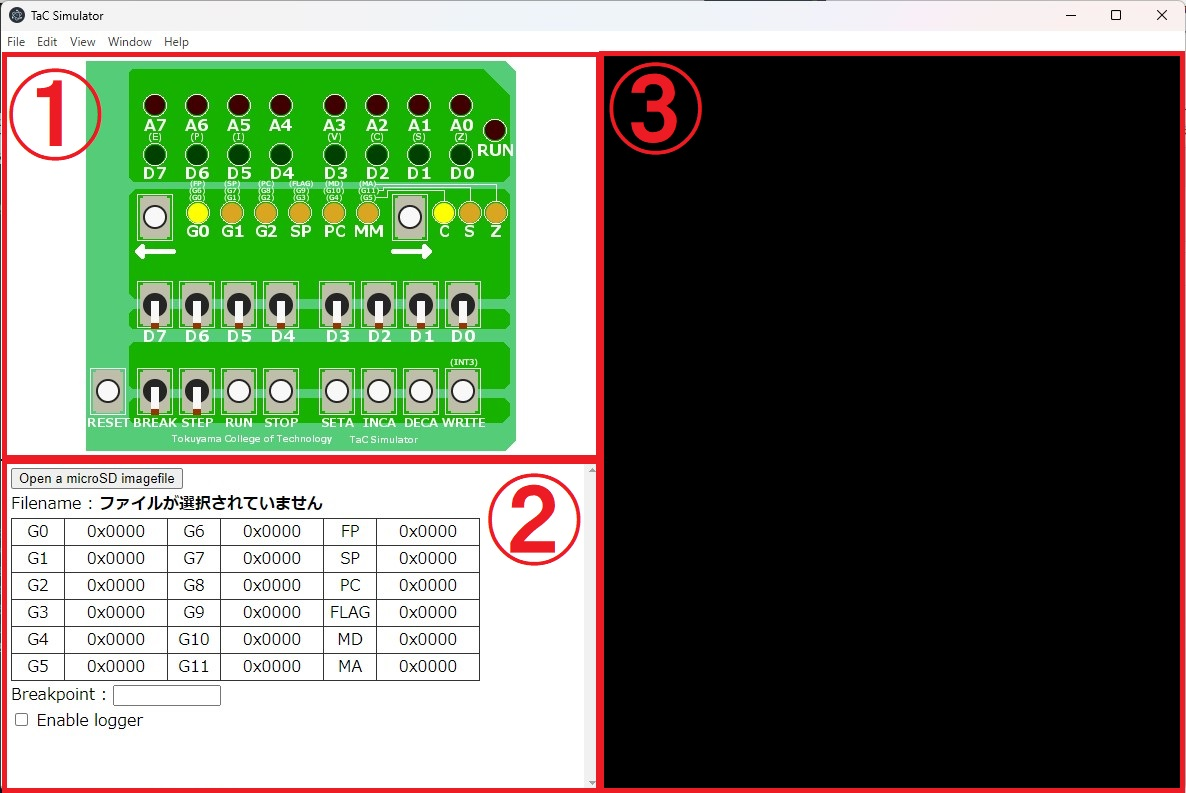
\includegraphics[width=12cm]{"figs/chapter3-tacsimulator.jpg"}
    \caption{\tacsim の画面} \label{fig:ch3-tacsim}
\end{figure}

\section{イメージファイルの実行}

コンソールのRUNボタンをクリックすることで, シミュレータに予め書き込まれているIPLプログラムが起動する. ただし, 初期状態ではマイクロSDが読み込まれていないため, ターミナルに次のような表示を出力して動作を停止する.

\begin{mylist}
\begin{verbatim}
TaC Initial Program Loader Ver.4.5.0(TeC7d v2.0.0)
(build date : Fri Oct 7 15:16:36 JST 2022)
Copyright(c) 2009-2022 Tokuyama College of Technology
All rights reserved.

Please insert the card.
Push "RESET" to boot the kernel
\end{verbatim}
\end{mylist}

\tacsim ではマイクロSDの代わりにFAT16ファイルシステムでフォーマットされたディスクイメージファイルを使用できる(以後, マイクロSDイメージファイルと呼ぶ). TacSimulator-TS/sampleディレクトリに入っているサンプル用のマイクロSDイメージファイルを使用することができる. また, 自分で作成することもできる(マイクロSDイメージファイルの作成方法は付録\ref{appA}参考).

「Open a microSD imagefile」ボタンをクリックすると, マイクロSDイメージファイルを選択するウィンドウが開く. 初期状態では拡張子が「.dmg」のファイルを選択するようになっているが, FAT16でフォーマットされたイメージファイルであれば, 拡張子の種類は問わない.

ファイルを選択した後, 図\ref{fig:ch3-filepath}のようにボタンの下の「Filename」に選択したファイルのパスが表示されたら, ファイルのオープンに成功している. この状態で再度コンソールのRUNボタンをクリックすると, IPLがマイクロSDイメージファイルを読み込み, 「kernel.bin」という名前で保存されているファイルをカーネルファイルとして実行する.

\begin{figure}[H]
    \centering
    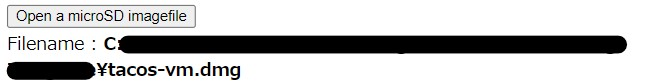
\includegraphics[width=12cm]{"figs/chapter3-filepath.jpg"}
    \caption{ファイルがオープンされている状態} \label{fig:ch3-filepath}
\end{figure}


\section{デバッグ機能}

\subsection{ステップ実行}
実機と同じようにステップ実行を行うことができる. コンソールのSTEPスイッチを上に上げた状態でRUNボタンをクリックすると1命令ずつ実行される.

\subsection{ブレークポイントの設定}
\tacsim では, レジスタ表示の下にある入力ボックスにブレークしたい命令のアドレスを16進数で入力することで設定することで, ブレークポイントの設定ができる. 
ブレークポイントを設定した後, コンソールのBREAKスイッチを上に上げた状態でRUNボタンをクリックすると指定した番地の命令を実行した後に停止する. 実機では指定した番地へのメモリアクセスの際に停止するが, \tacsim では仕様が異なる.

\subsection{レジスタの内容表示}
\tacsim ではレジスタの内容を16進数で表示している. 実機と同じようにロータリースイッチでレジスタを選択し, LEDランプで値を表示することも可能である. 表示しているレジスタの情報は, \tacsim がSTOP状態になったときに更新される. 

\subsection{開発者ツールのコンソールへの出力}

\tac 実機はUSBシリアル通信モジュールとBluetoothモジュールが接続されており, 接続相手のPCの都合に合わせて, どちらかを選択してターミナルとシリアル通信を行うことができる. \tacsim ではUSBシリアルと接続されたターミナルが表示されているので, Bluetoothシリアルはブラウザの開発者ツールのコンソールに接続する.
\tacos は, デバッグモードのとき通常の出力をUSBシリアルに, デバッグ用メッセージをBluetoothシリアルに出力するので, \tacsim でデバッグを行う際にはこの機能を使用できる.

この機能を有効にするには, 「Enable logger」の横のチェックボックスをクリックする.
画面上部のメニューバーから「View」\rightarrow 「Toggle Developer Tools」を選択することで, 開発者ツールが開く. 「Console」に移動してからRUNボタンをクリックすると, 出力が開発者ツールのコンソールにも出力されていることが確認できる.

\begin{figure}[H]
    \centering
    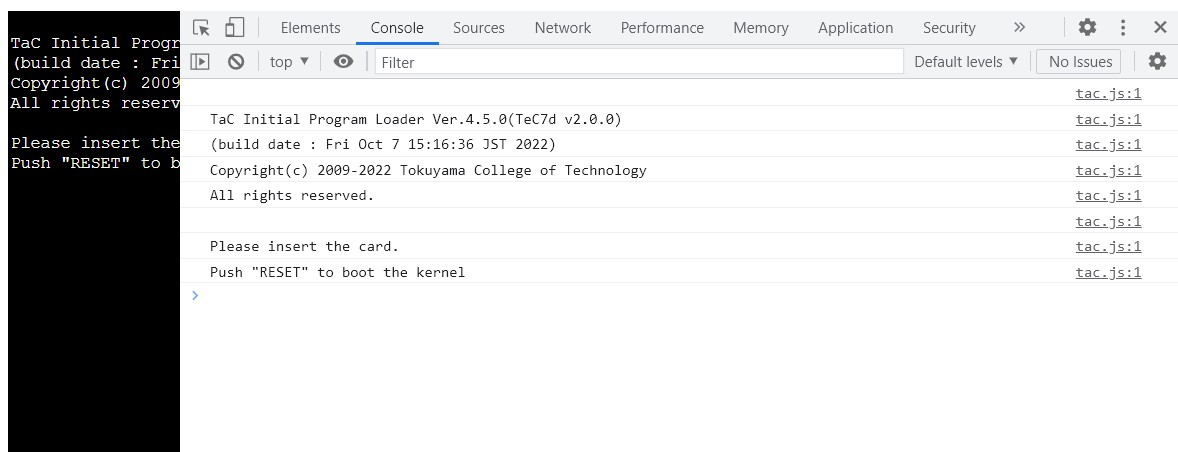
\includegraphics[width=14cm]{"figs/chapter3-devtools.jpg"}
    \caption{開発者ツールのコンソールへの出力} \label{fig:ch3-devtools}
\end{figure}

\section{試験的機能}

ここで紹介する機能は研究のデータ収集用に簡易的に作られたものである.

\subsection{TLBエントリ拡張}

TLBの数とメモリアクセスの速度の関係を調べるために, IOマップの0x60から0x7eにTLBエントリを8個新設している. \tacos 側で使用するエントリ数を変更すれば全てのエントリを使用するようになる.

\subsection{命令の実行回数・TLBMissの発生回数の計測}

この機能はdebugmodeブランチで実装している.

指定したプロセス番号で命令が何回実行されているか, あるいはTLBMissは何回発生しているかを計測することができる. \textgt{この機能を使用するには, \tacos がプロセスをディスパッチする際にプロセス番号をI/Oの0x38番地に書き込むように修正する必要がある.}

\begin{figure}[H]
    \centering
    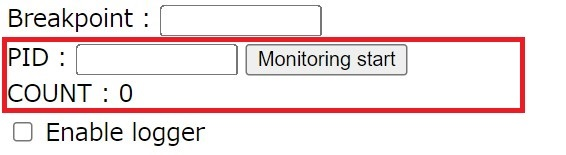
\includegraphics[width=9cm]{"figs/chapter3-monitor.jpg"}
    \caption{開発者ツールのコンソールへの出力} \label{fig:ch3-monitor}
\end{figure}

PIDに計測したいプロセス番号を入力し, 「Monitoring start」ボタンをクリックすると計測が開始される. もう一度ボタンを押すと, それまでの命令の実行回数とTLBMissの発生回数が表示される. 図\ref{fig:ch3-monitor2}では, \tacos のlsコマンドの命令の実行回数とTLBMissの発生回数を計測している様子である.

\begin{figure}[H]
    \centering
    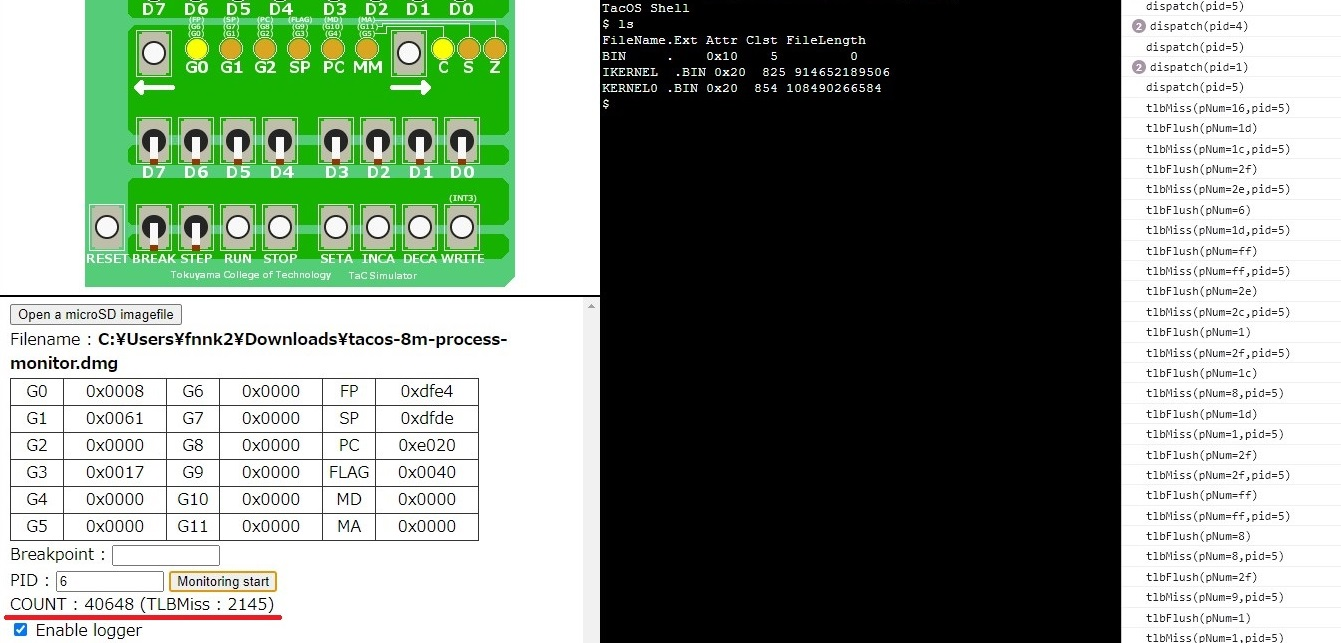
\includegraphics[width=14cm]{"figs/chapter3-monitor2.jpg"}
    \caption{実行回数計測の様子} \label{fig:ch3-monitor2}
\end{figure}